% \clearpage
\maketitlesupplementary

\newtheorem{lemma}{Lemma}
\setcounter{page}{1}
\setcounter{section}{0}
\setcounter{table}{0}
\setcounter{figure}{0}
\setcounter{equation}{0}

\renewcommand{\thefigure}{A\arabic{figure}} % set caption label style
\renewcommand{\thetable}{A\arabic{table}} 
\renewcommand{\thesection}{A\arabic{section}} 
\renewcommand{\thesubsection}{A\arabic{subsection}} 

% \onecolumn

\section{Theoretical Analysis}
% \textbf{Lemma 1 (Cycle-consistency, Universe Matching).} 
\begin{lemma}[Cycle-consistency, Universe Matching]
Given a set of pairwise (partial) matching matrices $\{\mathbf{X}_{ij}\}_{i,j=1}^m$, it is cycle-consistent iff there exists a collection of universe matching matrices \(\{ U_i \in \mathbb{U}_{n_i, d} \}_{i=1}^m\) such that for each graph pair $(\mathcal{G}_i, \mathcal{G}_j)$, we have
\begin{equation}
    \mathbf{X}_{ij} = U_i U_j^{\mathsf{T}}.\nonumber
\end{equation}
\end{lemma}

% \textbf{Proof:}
\begin{proof}
We need to prove that the matching matrices $\{\mathbf{X}_{ij}\}_{i,j=1}^m$ satisfy cycle-consistency, which means that:
\begin{equation}
    \mathbf{X}_{ij} \mathbf{X}_{jk} = \mathbf{X}_{ik}. \forall i, j, k\in [m]
\end{equation}
 
By the assumption of the \textit{lemma 1}, there exists a collection of universe matching matrices $\{ U_i \}_{i=1}^m$ such that for each pair $(\mathcal{G}_i, \mathcal{G}_j)$,
\begin{equation}
    \mathbf{X}_{ij} = U_i U_j^{\mathsf{T}}.
\end{equation}
Therefore, we have
\begin{equation}
    \mathbf{X}_{ij} = U_i U_j^{\mathsf{T}}, \quad \mathbf{X}_{jk} = U_j U_k^{\mathsf{T}}, \quad \mathbf{X}_{ik} = U_i U_k^{\mathsf{T}}.
\end{equation}
Now we compute $\mathbf{X}_{ij} \mathbf{X}_{jk}$:
\begin{align}
    \mathbf{X}_{ij} \mathbf{X}_{jk} &= (U_i U_j^{\mathsf{T}})(U_j U_k^{\mathsf{T}}) \nonumber \\ 
    &= U_i (U_j^{\mathsf{T}} U_j) U_k^{\mathsf{T}}. 
    \label{eq.6}
\end{align}

Assume that each matrix $U_i$ satisfies $U_i^{\mathsf{T}} U_i = I$ (i.e., $U_i$ is an orthogonal matrix or has unit inner product property). 
Thus, Eq. (\ref{eq.6}) simplifies further to:
\begin{equation}
    \mathbf{X}_{ij} \mathbf{X}_{jk} = U_i I U_k^{\mathsf{T}} = U_i U_k^{\mathsf{T}} = \mathbf{X}_{ik}.
\end{equation}

This shows that the matching matrices $\{\mathbf{X}_{ij}\}_{i,j=1}^m$ satisfy cycle-consistency. 
\end{proof}


\section{Algorithm Pipeline}
\label{sec:algo}
Algorithms~\ref{algo:train} and \ref{algo:test} outline the procedures for the source training phase and the test-time adaptation phase, respectively, while Algorithm~\ref{algo:hippi} provides a detailed explanation of the HiPPI~\cite{bernard2019hippi} method used in Algorithm~\ref{algo:train}.

\section{Additional Experiments}
\subsection{Single Source DG in Retinal Fundus}
\begin{table*}[h!]
% \vspace{-9pt}
% \setlength{\tabcolsep}{1pt}
\centering
  \caption{Single source domain generalization in the retinal fundus segmentation. The performance (mean $\pm$ standard deviation) of three trials for our method and eight SOTA methods. ``A $\rightarrow \{B,C,D,E\}$'' represents models trained on Site A and tested on the mixed distribution of Sites B-E, and similar for others. Best results are colored as \textcolor{red}{red}.}
  % \vspace{-10pt}
  \begin{adjustbox}{width=0.99\linewidth}
    % \begin{tabular}{c|cccccccccccccccccccc|c}
% \hlineB{3}
% \multirow{2}{*}{Methods}  
% & A $\rightarrow$ B & A $\rightarrow$ C & A $\rightarrow$ D & A $\rightarrow$ E & B $\rightarrow$ A & B $\rightarrow$ C & B $\rightarrow$ D & B $\rightarrow$ E & C $\rightarrow$ A & C $\rightarrow$ B & C $\rightarrow$ D & C $\rightarrow$ E & D $\rightarrow$ A & D $\rightarrow$ B & D $\rightarrow$ C & D $\rightarrow$ E & E $\rightarrow$ A & E $\rightarrow$ B & E $\rightarrow$ C & E $\rightarrow$ D & Avg. \\  \cline{2-22}

% & \multicolumn{21}{c}{\textbf{Dice Score Metric $\uparrow$ }} \\ \hline \hline

% \textit{No Adapt} (U-Net~\cite{ronneberger2015u}) & - & - & - & - & - & - & - & - & - & - & - & - & - & - & - & - & - & - & - & - & - \\ \hline
% TENT (ICLR'21)~\cite{wangtent} & - & - & - & - & - & - & - & - & - & - & - & - & - & - & - & - & - & - & - & - & - \\
% TASD (AAAI'22)~\cite{liu2022single} & - & - & - & - & - & - & - & - & - & - & - & - & - & - & - & - & - & - & - & - & - \\
% DLTTA (TMI'22)~\cite{yang2022dltta} & - & - & - & - & - & - & - & - & - & - & - & - & - & - & - & - & - & - & - & - & - \\
% SAR (ICLR'23)~\cite{niu2023towards} & - & - & - & - & - & - & - & - & - & - & - & - & - & - & - & - & - & - & - & - & - \\
% DomainAdaptor (CVPR'23)~\cite{zhang2023domainadaptor} & - & - & - & - & - & - & - & - & - & - & - & - & - & - & - & - & - & - & - & - & - \\
% DeY-Net (WACV'24)~\cite{wen2024denoising} & - & - & - & - & - & - & - & - & - & - & - & - & - & - & - & - & - & - & - & - & - \\
% VPTTA (CVPR'24)~\cite{chen2024each} & - & - & - & - & - & - & - & - & - & - & - & - & - & - & - & - & - & - & - & - & - \\ 
% NC-TTT (CVPR'24)~\cite{osowiechi2024nc} & - & - & - & - & - & - & - & - & - & - & - & - & - & - & - & - & - & - & - & - & - \\ \hline
% Ours & - & - & - & - & - & - & - & - & - & - & - & - & - & - & - & - & - & - & - & - & - \\ \hlineB{3}
% \end{tabular}


\begin{tabular}{c|ccccccccccccccc|ccc}
\hlineB{3}
\multirow{2}{*}{Methods} & \multicolumn{3}{c}{A $\rightarrow \{B,C,D,E\}$} & \multicolumn{3}{c}{B $\rightarrow  \{A,C,D,E\}$} & \multicolumn{3}{c}{C $\rightarrow  \{A,B,D,E\}$} & \multicolumn{3}{c}{D $\rightarrow  \{A,B,C,E\}$} & \multicolumn{3}{c|}{E $\rightarrow  \{A,B,C,D\}$} & \multicolumn{3}{c}{Average} \\ \cline{2-19} 
                         & \textit{DSC}       & $E_\phi^{max}$       & $S_{\alpha}$      & \textit{DSC}       & $E_\phi^{max}$       & $S_{\alpha}$     & \textit{DSC}       & $E_\phi^{max}$       & $S_{\alpha}$    & \textit{DSC}       & $E_\phi^{max}$       & $S_{\alpha}$  & \textit{DSC}       & $E_\phi^{max}$       & $S_{\alpha}$      & \textit{DSC} $\uparrow$      & $E_\phi^{max}$ $\uparrow$       & $S_{\alpha}$ $\uparrow$    \\ \hline \hline
\textit{No Adapt} (U-Net~\cite{ronneberger2015u}) &70.60\small{$\pm$10.01} & 86.92\small{$\pm$1.17} & 80.36\small{$\pm$0.88} & 77.08\small{$\pm$6.90} & 91.58\small{$\pm$0.84} & 85.44\small{$\pm$0.99} & 66.24\small{$\pm$8.45} & 86.49\small{$\pm$0.77} & 80.01\small{$\pm$0.91} & 71.21\small{$\pm$9.47} & 82.90\small{$\pm$1.48} & 80.11\small{$\pm$0.88} & 72.26\small{$\pm$7.60} & 86.51\small{$\pm$1.02} & 86.05\small{$\pm$0.68} & 71.47 & 86.88 & 82.39\\ \hline
% TENT (ICLR'21)~\cite{wangtent}   \\
TASD (AAAI'22)~\cite{liu2022single} & 79.89\small{$\pm$5.91} & 93.26\small{$\pm$0.21} & 87.12\small{$\pm$0.13} & 82.63\small{$\pm$3.24} & 93.20\small{$\pm$0.25} & 86.00\small{$\pm$0.10} & 78.03\small{$\pm$4.29} & 92.47\small{$\pm$0.14} & 86.71\small{$\pm$0.09} & 76.30\small{$\pm$7.81} & 86.09\small{$\pm$0.15} & 80.94\small{$\pm$0.11} & 79.99\small{$\pm$1.29} & 93.24\small{$\pm$0.10} & 87.08\small{$\pm$0.08} & 79.36 & 91.65 & 85.57  \\
% CoTTA (CVPR'22)~\cite{wang2022continual}       \\

DLTTA (TMI'22)~\cite{yang2022dltta} & 74.96\small{$\pm$7.20} & 89.24\small{$\pm$0.25} & 84.02\small{$\pm$0.11} & 78.27\small{$\pm$5.66} & 92.40\small{$\pm$0.40} & 85.36\small{$\pm$0.11} & 75.84\small{$\pm$5.14} & 90.96\small{$\pm$0.20} & 84.11\small{$\pm$0.10} & 65.55\small{$\pm$9.35} & 84.80\small{$\pm$0.18} & 78.33\small{$\pm$0.08} & 71.68\small{$\pm$4.99} & 87.79\small{$\pm$0.17} & 85.13\small{$\pm$0.09} & 73.26 & 89.03 & 83.39\\

SAR (ICLR'23)~\cite{niu2023towards} & 74.20\small{$\pm$6.09} & 89.07\small{$\pm$0.33} & 83.64\small{$\pm$0.10} & 80.34\small{$\pm$2.86} & 92.70\small{$\pm$0.41} & 85.95\small{$\pm$0.12} & 72.58\small{$\pm$4.46} & 91.20\small{$\pm$0.20} & 83.47\small{$\pm$0.09} & 70.30\small{$\pm$8.98} & 85.10\small{$\pm$1.09} & 79.42\small{$\pm$0.72} & 70.31\small{$\pm$5.77} & 88.56\small{$\pm$0.81} & 86.79\small{$\pm$0.30} & 73.54 & 89.32 & 83.85\\

DomainAdaptor (CVPR'23)~\cite{zhang2023domainadaptor} & 77.23\small{$\pm$3.97} & 90.22\small{$\pm$0.40} & 84.20\small{$\pm$0.11} & 76.41\small{$\pm$4.28} & 91.80\small{$\pm$0.31} & 85.73\small{$\pm$0.12} & 70.17\small{$\pm$8.01} & 91.32\small{$\pm$0.24} & 83.50\small{$\pm$0.09} & 67.39\small{$\pm$9.82} & 84.16\small{$\pm$0.21} & 78.02\small{$\pm$0.08} & 76.97\small{$\pm$4.59} & 89.30\small{$\pm$0.13} & 85.46\small{$\pm$0.08} & 73.63 & 89.36 & 83.38 \\

DeY-Net (WACV'24)~\cite{wen2024denoising} 
 & 80.03\small{$\pm$8.31} &94.42\small{$\pm$0.20} & 86.35\small{$\pm$0.84} & {84.30\small{$\pm$7.09}} & \textcolor{red}{94.25\small{$\pm$0.23}} & \textcolor{red}{87.16\small{$\pm$0.47}} & 80.32\small{$\pm$7.85} & 93.40\small{$\pm$0.32} & 88.41\small{$\pm$0.33} & 78.67\small{$\pm$5.31} & 86.12\small{$\pm$0.78} & 80.45\small{$\pm$0.30} & 76.81\small{$\pm$3.79} &90.09\small{$\pm$0.55} & 86.30\small{$\pm$0.25} & 80.02 & 91.65&85.73\\

VPTTA (CVPR'24)~\cite{chen2024each} &73.57\small{$\pm$6.60} & 92.68\small{$\pm$0.03} & 84.14\small{$\pm$0.01} & 78.21\small{$\pm$2.40} & 94.07\small{$\pm$0.09} & 86.16\small{$\pm$0.01} & 69.26\small{$\pm$4.29} & 92.78\small{$\pm$0.08} & 82.66\small{$\pm$0.02} & 60.11\small{$\pm$8.05} & 85.18\small{$\pm$0.10} & 76.24\small{$\pm$0.03} & 72.58\small{$\pm$5.21} & 91.16\small{$\pm$0.13} & 84.74\small{$\pm$0.04} & 70.74 & 91.17 & 82.78\\ 

NC-TTT (CVPR'24)~\cite{osowiechi2024nc} & 78.21\small{$\pm$2.74} & 93.87\small{$\pm$0.25} & 85.49\small{$\pm$0.11} & 82.13\small{$\pm$3.30} & 93.19\small{$\pm$0.29} & 86.78\small{$\pm$0.08} & 77.50\small{$\pm$5.29} & 91.99\small{$\pm$0.14} & 84.08\small{$\pm$0.03} & 74.14\small{$\pm$3.50} & 87.53\small{$\pm$0.25} & 80.56\small{$\pm$0.11} & 80.53\small{$\pm$1.08} & 92.73\small{$\pm$0.10} & 85.81\small{$\pm$0.07} & 78.50 & 91.86 & 84.54
  \\  

% MedBN (CVPR'24)~\cite{park2024medbn} \\
\hline

Ours & \textcolor{red}{85.25\small{$\pm$2.33}} &  \textcolor{red}{94.68\small{$\pm$0.09}} & \textcolor{red}{88.52\small{$\pm$0.13}} & \textcolor{red}{85.34\small{$\pm$3.08}} & 93.18\small{$\pm$0.20} & 86.83\small{$\pm$0.11} & \textcolor{red}{86.19\small{$\pm$1.99}} & \textcolor{red}{94.57\small{$\pm$0.20}} & \textcolor{red}{89.24\small{$\pm$0.13}} & \textcolor{red}{81.52\small{$\pm$4.25}} & \textcolor{red}{91.20\small{$\pm$0.30}} & \textcolor{red}{84.53\small{$\pm$0.28}} & \textcolor{red}{86.08\small{$\pm$3.08}} & \textcolor{red}{94.60\small{$\pm$0.23}} & \textcolor{red}{88.58\small{$\pm$0.11}} & \textcolor{red}{84.87} & \textcolor{red}{93.64} & \textcolor{red}{87.54} \\ 

\hlineB{3}
\end{tabular}

  \end{adjustbox}
  \label{tab:tabel_single_fundus}
\end{table*}

For the retinal fundus segmentation task, we conducted single-source domain generalization experiments. Unlike the experiments described in the main text, this setup simulates a more realistic scenario where test data may originate from arbitrarily complex real-world distributions, i.e., mixed distribution shifts. Specifically, data from one site was selected and split $8:2$ into training and validation sets ($S=1$), while the remaining sites ($T=|\mathcal{D}_s \cup \mathcal{D}_t|-1$) were shuffled and used entirely as the testing dataset. Notably, all models encountered these target domains for the first time during testing.

As shown in Table~\ref{tab:tabel_single_fundus}, our approach achieved SOTA performance across all five transfer experiments for the DSC metric. In the average results, we outperformed the second-best method (DeY-Net~\cite{wen2024denoising}) by 4.85\%, 1.78\%, and 1.81\% in the DSC, $E_\phi^{max}$, and $S_{\alpha}$, respectively. These results validate the effectiveness of our method for medical image segmentation tasks.
        
The retinal fundus dataset is characterized by significant low-level visual differences and features segmentation targets that are not singular, often exhibiting overlapping and fixed structures. We attribute our superior performance to the comprehensive learning of the morphological knowledge of organs. This enables our method to robustly distinguish organ instances and their shape features—a domain-invariant property—even under severe domain shifts that degrade the performance of other methods.

\subsection{Multi Source DG in MRI Prostate}
\noindent \textbf{Datasets.}
We conducted experiments on the prostate segmentation task using T2-weighted MRI scans collected from six different clinical centers, denoted as Domain RUNMC, BMC, I2CVB, UCL, BIDMC, and HK. These centers are sourced from three publicly available datasets: NCI-ISBI13~\cite{nicholas2015nci}, I2CVB~\cite{lemaitre2015computer}, and PROMISE12~\cite{litjens2014evaluation}.

\noindent \textbf{Implementation Details.}
We followed the data preprocessing pipeline of \cite{zhang2024pass} to ensure consistency. Specifically, we used 30 labeled cases from RUNMC as the source dataset and evaluated the model on 30, 19, 13, 12, and 12 unlabeled cases from the five remaining clinical sites. Each MRI axial slice was resized to $384 \times 384$ pixels and normalized to have zero mean and unit variance. Before normalization, we clipped the 5\%–95\% intensity range of the histograms to reduce outlier influence.

For feature extraction, we employed a ResNet-50 backbone pre-trained on ImageNet. During both the source model training and test-time adaptation (TTA) stages, we maintained a batch size of 8.
Given that edge precision is crucial in MRI prostate segmentation, and considering the complex shape variations of the prostate, we selected Dice Score (DSC) and Hausdorff Distance (HD95) as the primary evaluation metrics to provide a comprehensive performance assessment.

\noindent \textbf{Experimental Results.}
\begin{table*}[h!]
% \vspace{-9pt}
% \setlength{\tabcolsep}{1pt}
\centering
  \caption{Test-time domain generalization results on the MRI prostate datasets.  The performance (mean $\pm$ standard deviation) of three trials for our method and six SOTA methods. Best results are colored as \textcolor{red}{red}.}
  % \vspace{-10pt}
  \begin{adjustbox}{width=0.969\linewidth}
    \begin{tabular}{c|cccccccccc|cc}
\hlineB{3}
\multirow{2}{*}{Methods} & \multicolumn{2}{c}{BMC} & \multicolumn{2}{c}{I2CVB} & \multicolumn{2}{c}{UCL} & \multicolumn{2}{c}{BIDMC}  & \multicolumn{2}{c|}{HK} & \multicolumn{2}{c}{Avg.}   \\ \cline{2-13} 
                         & \textit{DSC}      &  HD95    & \textit{DSC}      &  HD95& \textit{DSC}      &  HD95& \textit{DSC}     &  HD95  & \textit{DSC}      &  HD95  & \textit{DSC} $\uparrow$     &  HD95 $\downarrow$ \\ \hline \hline

\textit{No Adapt} & 74.30\small{$\pm$5.31} & 16.08\small{$\pm$12.41} & 66.47\small{$\pm$13.50} & 37.16\small{$\pm$18.24} & 75.28\small{$\pm$6.20} & 16.77\small{$\pm$12.10} & 52.08\small{$\pm$7.71} & 50.09\small{$\pm$20.85} & 80.51\small{$\pm$9.35} & 8.79\small{$\pm$9.06} & 69.72\small{$\pm$8.29} & 25.77\small{$\pm$15.41}  \\  \hline

TENT (ICLR'21)~\cite{wangtent} & 77.45\small{$\pm$3.79} & 12.09\small{$\pm$9.88} & 69.10\small{$\pm$10.47} & 30.78\small{$\pm$19.22} & 79.69\small{$\pm$4.81} & 14.71\small{$\pm$11.01} & 52.01\small{$\pm$6.80} & 42.63\small{$\pm$10.13} & 84.58\small{$\pm$2.73} & 4.07\small{$\pm$5.38} & 72.56\small{$\pm$4.26} & 20.85\small{$\pm$13.64} \\

TASD (AAAI'22)~\cite{liu2022single} & 76.28\small{$\pm$2.35} & 15.11\small{$\pm$15.17} & 68.30\small{$\pm$7.88} & 31.43\small{$\pm$24.10} & 80.25\small{$\pm$3.54} & \textcolor{red}{10.59\small{$\pm$16.39}} & 56.08\small{$\pm$3.82} & 51.90\small{$\pm$24.82} & 81.09\small{$\pm$1.79} & 4.26\small{$\pm$4.16} & 72.40\small{$\pm$5.72} & 22.65\small{$\pm$17.53}  \\

SAR (ICLR'23)~\cite{niu2023towards} & 77.24\small{$\pm$4.26} & 20.48\small{$\pm$10.12} & 68.99\small{$\pm$8.27} & 49.07\small{$\pm$15.66} & 79.27\small{$\pm$8.48} & 18.03\small{$\pm$5.89} & 50.81\small{$\pm$10.60} & 54.35\small{$\pm$19.31} & 85.40\small{$\pm$3.08} & 3.87\small{$\pm$3.55} & 72.34\small{$\pm$4.80} & 29.16\small{$\pm$16.28} \\

DomainAdaptor (CVPR'23)~\cite{zhang2023domainadaptor} & 76.49\small{$\pm$2.59} & 19.27\small{$\pm$8.13} & 69.07\small{$\pm$9.14} & 32.57\small{$\pm$10.40} & 80.41\small{$\pm$5.08} & 16.24\small{$\pm$9.88} & 49.99\small{$\pm$14.28} & 48.40\small{$\pm$10.28} & 85.20\small{$\pm$1.90} & 3.25\small{$\pm$6.94} & 72.23\small{$\pm$6.82} & 23.94\small{$\pm$14.55} \\

VPTTA (CVPR'24)~\cite{chen2024each}& 77.42\small{$\pm$4.38} & 12.93\small{$\pm$7.09} & 70.25\small{$\pm$5.18} & 30.01\small{$\pm$13.68} 
 & 82.07\small{$\pm$6.27} & 13.28\small{$\pm$18.09} & 57.49\small{$\pm$8.46} & 40.11\small{$\pm$12.05} & 83.27\small{$\pm$2.96} & 3.40\small{$\pm$5.45} & 74.10\small{$\pm$4.79} & 19.94\small{$\pm$12.99}   \\

PASS (TMI'24)~\cite{zhang2024pass} & \textcolor{red}{80.07\small{$\pm$7.14}} & 10.50\small{$\pm$9.57} &71.41\small{$\pm$6.28} & 28.26\small{$\pm$9.97} & 84.39\small{$\pm$8.81} & 10.68\small{$\pm$12.27} & 57.27\small{$\pm$11.48} & \textcolor{red}{36.94\small{$\pm$16.43}} & 84.88\small{$\pm$3.71} & 3.03\small{$\pm$5.05} & 75.60\small{$\pm$5.13} & 17.88\small{$\pm$12.14} \\ \hline

Ours & 79.63\small{$\pm$4.71} & \textcolor{red}{9.99\small{$\pm$11.10}} & \textcolor{red}{74.09\small{$\pm$9.80}} & \textcolor{red}{25.70\small{$\pm$13.07}} & \textcolor{red}{86.30\small{$\pm$7.25}} & 11.08\small{$\pm$17.47} & \textcolor{red}{60.33\small{$\pm$13.59}} & 39.52\small{$\pm$14.20}  & \textcolor{red}{86.12\small{$\pm$2.08}} & \textcolor{red}{2.84\small{$\pm$8.08}} & \textcolor{red}{77.29\small{$\pm$3.98}} & \textcolor{red}{17.82\small{$\pm$11.06}}  \\



\hlineB{3}
\end{tabular}

  \end{adjustbox}
  \label{tab:tabel_prostate}
\end{table*}
The MRI prostate segmentation results are presented in Table~\ref{tab:tabel_prostate}, where we compare our method against several SOTA approaches, including the latest TTA segmentation method, PASS~\cite{zhang2024pass}.
As shown in the results, the performance of existing TTA methods remains relatively close across both DSC and HD95 metrics. While PASS exhibits strong segmentation performance, our method surpasses it with a 1.69\% improvement in DSC, demonstrating its effectiveness.
Given the inherent challenges of MRI prostate segmentation, characterized by diverse imaging modalities and complex morphological variations, our results highlight the robust generalization capability of our approach. Nonetheless, further enhancing edge precision remains an important focus for our future work.

\subsection{Natural Image Classification}
\noindent \textbf{Datasets.} For natural image classification tasks, we selected two benchmark datasets: PACS~\cite{li2017deeper} and VLCS~\cite{fang2013unbiased}, which are widely used in domain generalization and test-time adaptation studies. 
The PACS~\cite{li2017deeper} dataset consists of large images spanning 7 classes evenly distributed across 4 domains, i.e. A (Art), C (Cartoons), P (Photos), and S (Sketches), with a total of 9,991 images. 
The VLCS~\cite{fang2013unbiased} dataset comprises 10,729 images across 5 classes (bird, car, chair, dog, and person), evenly distributed across 4 domains: C (Caltech101), L (LabelMe), S (SUN09), and V (VOC2007).

\noindent \textbf{Source model training.} For all experiments, we employed an ImageNet-pretrained ResNet-50~\cite{he2016deep} as the feature extractor, with an MLP layer provided by the DomainBed~\cite{gulrajanisearch} benchmark serving as the classifier. We used the SGD optimizer with a learning rate of $1 \times 10^{-5}$. The batch size was set to 32, and training was conducted for 10,000 iterations. All images were resized to $224 \times 224$, and data augmentation techniques—including random cropping, flipping, color jittering, and intensity adjustments—were applied during source training.

\noindent \textbf{Implementation details of test-time adaptation setup.} We evaluated our framework against six methods (i.e. Empirical Risk Minimization (ERM)~\cite{vapnik1998statistical}, DomainAdaptor~\cite{zhang2023domainadaptor}, ITTA~\cite{chen2023improved}, VPTTA~\cite{chen2024each}, NC-TTT~\cite{osowiechi2024nc}) under fair comparison conditions, following the leave-one-out training strategy using the publicly available DomainBed~\cite{gulrajanisearch} framework. For deploying our framework at the test-time phase, we employed SGD with a learning rate of 0.005, a batch size of 16, and a universe size of $d = 60$. Notably, as all images in the natural image classification task contain only a single instance class, the class-wise similarity matrix described in Section 3.2 of the main text was not utilized.

\noindent \textbf{Experimental Results.} The classification results across different domains for natural images are presented in Tables~\ref{tab:tabel_natural_pacs} and \ref{tab:tabel_natural_vlcs}. While the ERM method shows strong performance compared to existing approaches, our method achieves higher classification accuracy, surpassing ERM by 3.01\% on the PACS dataset and 2.49\% on the VLCS dataset. Additionally, our approach demonstrates competitive performance against state-of-the-art test-time adaptation methods designed for natural images. Natural images present greater challenges compared to medical images due to the lack of consistent morphological priors typically observed in the latter. However, unlike segmentation tasks, classification does not require determining the specific class of every pixel in an image. Our framework’s graph construction effectively captures spatial correspondences for each instance, further enhancing its performance.

\begin{table}[h!]
% \vspace{-9pt}
% \setlength{\tabcolsep}{1pt}
\centering
  \caption{Test-time domain generalization results on the PACS~\cite{li2017deeper} dataset using a ResNet-50 backbone. Each column (A, C, P, S) indicates the domain used as the test set, while the remaining domains are used for training. The best results are highlighted in \textcolor{red}{red}.}
  % \vspace{-10pt}
  \begin{adjustbox}{width=0.969\linewidth}
    \begin{tabular}{c|ccccc}
    \hlineB{3}
        Method & A & C & P & S & Avg. \\ \hline
        ERM~\cite{vapnik1998statistical} & 84.07 & 80.21 & 97.06 & 81.99 & 85.83 \\ \hline
        TENT (ICLR'21)~\cite{wangtent} & 82.34 & 78.63 & 97.93 & 82.72 & 85.40 \\ 
        DomainAdaptor (CVPR'23)~\cite{zhang2023domainadaptor} & 86.15 & 82.02 & 98.40 & 84.38 & 88.45 \\ 
        ITTA (CVPR'23)~\cite{chen2023improved}& 85.63 & \textcolor{red}{84.30} & 97.27 & 84.09 & 87.82 \\
        VPTTA (CVPR'24)~\cite{chen2024each} & \textcolor{red}{86.50}  & 83.77 & 97.09 & 85.10 & 88.12 \\ 
        NC-TTT (CVPR'24)~\cite{osowiechi2024nc}& 83.81 & 80.44 & 96.53 & 82.36 & 85.79 \\ 
        Ours & 85.08 & 83.93 & \textcolor{red}{98.61} & \textcolor{red}{87.76} & \textcolor{red}{88.84} \\ \hlineB{3}
\end{tabular}
  \end{adjustbox}
  \label{tab:tabel_natural_pacs}
\end{table}

\begin{table}[h!]
% \vspace{-9pt}
% \setlength{\tabcolsep}{1pt}
\centering
  \caption{Test-time domain generalization results on the VLCS~\cite{fang2013unbiased} dataset using a ResNet-50 backbone. Each column (C, L, S, V) indicates the domain used as the test set, while the remaining domains are used for training. The best results are highlighted in \textcolor{red}{red}.}
  % \vspace{-10pt}
  \begin{adjustbox}{width=0.969\linewidth}
    \begin{tabular}{c|ccccc}
    \hlineB{3}
        Method & C & L & S & V & Avg. \\ \hline
        ERM~\cite{vapnik1998statistical} & 97.63 & 64.20 & 70.39 & 74.41 & 76.66 \\ \hline
        TENT (ICLR'21)~\cite{wangtent} & 96.88 & 64.46 & 71.07 & 73.52 & 76.48 \\ 
        DomainAdaptor (CVPR'23)~\cite{zhang2023domainadaptor} & \textcolor{red}{98.69} & \textcolor{red}{69.18} & 73.66 & 76.01 & \textcolor{red}{79.39} \\ 
        ITTA (CVPR'23)~\cite{chen2023improved}& 97.30 & 66.09 & 72.31 & 75.10 & 77.70 \\
        VPTTA (CVPR'24)~\cite{chen2024each} & 97.25  & 67.69 & 71.78 & 75.22 & 77.98 \\ 
        NC-TTT (CVPR'24)~\cite{osowiechi2024nc}& 96.72 & 65.58 & 73.04 & \textcolor{red}{76.83} & 78.04 \\ 
        Ours & 98.49 & 68.72 & \textcolor{red}{74.12} & 75.30 & 79.15 \\ \hlineB{3}
\end{tabular}
  \end{adjustbox}
  \label{tab:tabel_natural_vlcs}
\end{table}

\subsection{Additional Visualization}
We conducted additional visualization experiments, with segmentation results for retinal fundus and polyp images shown in Figures \ref{fig:vis_appendix_fundus} and \ref{fig:vis_appendix_poloy}, respectively. Each row represents images from a distinct domain (Site), and we ensured that the model performing inference had not encountered images from that domain before. 

\begin{figure*}[!t]
    \centering
    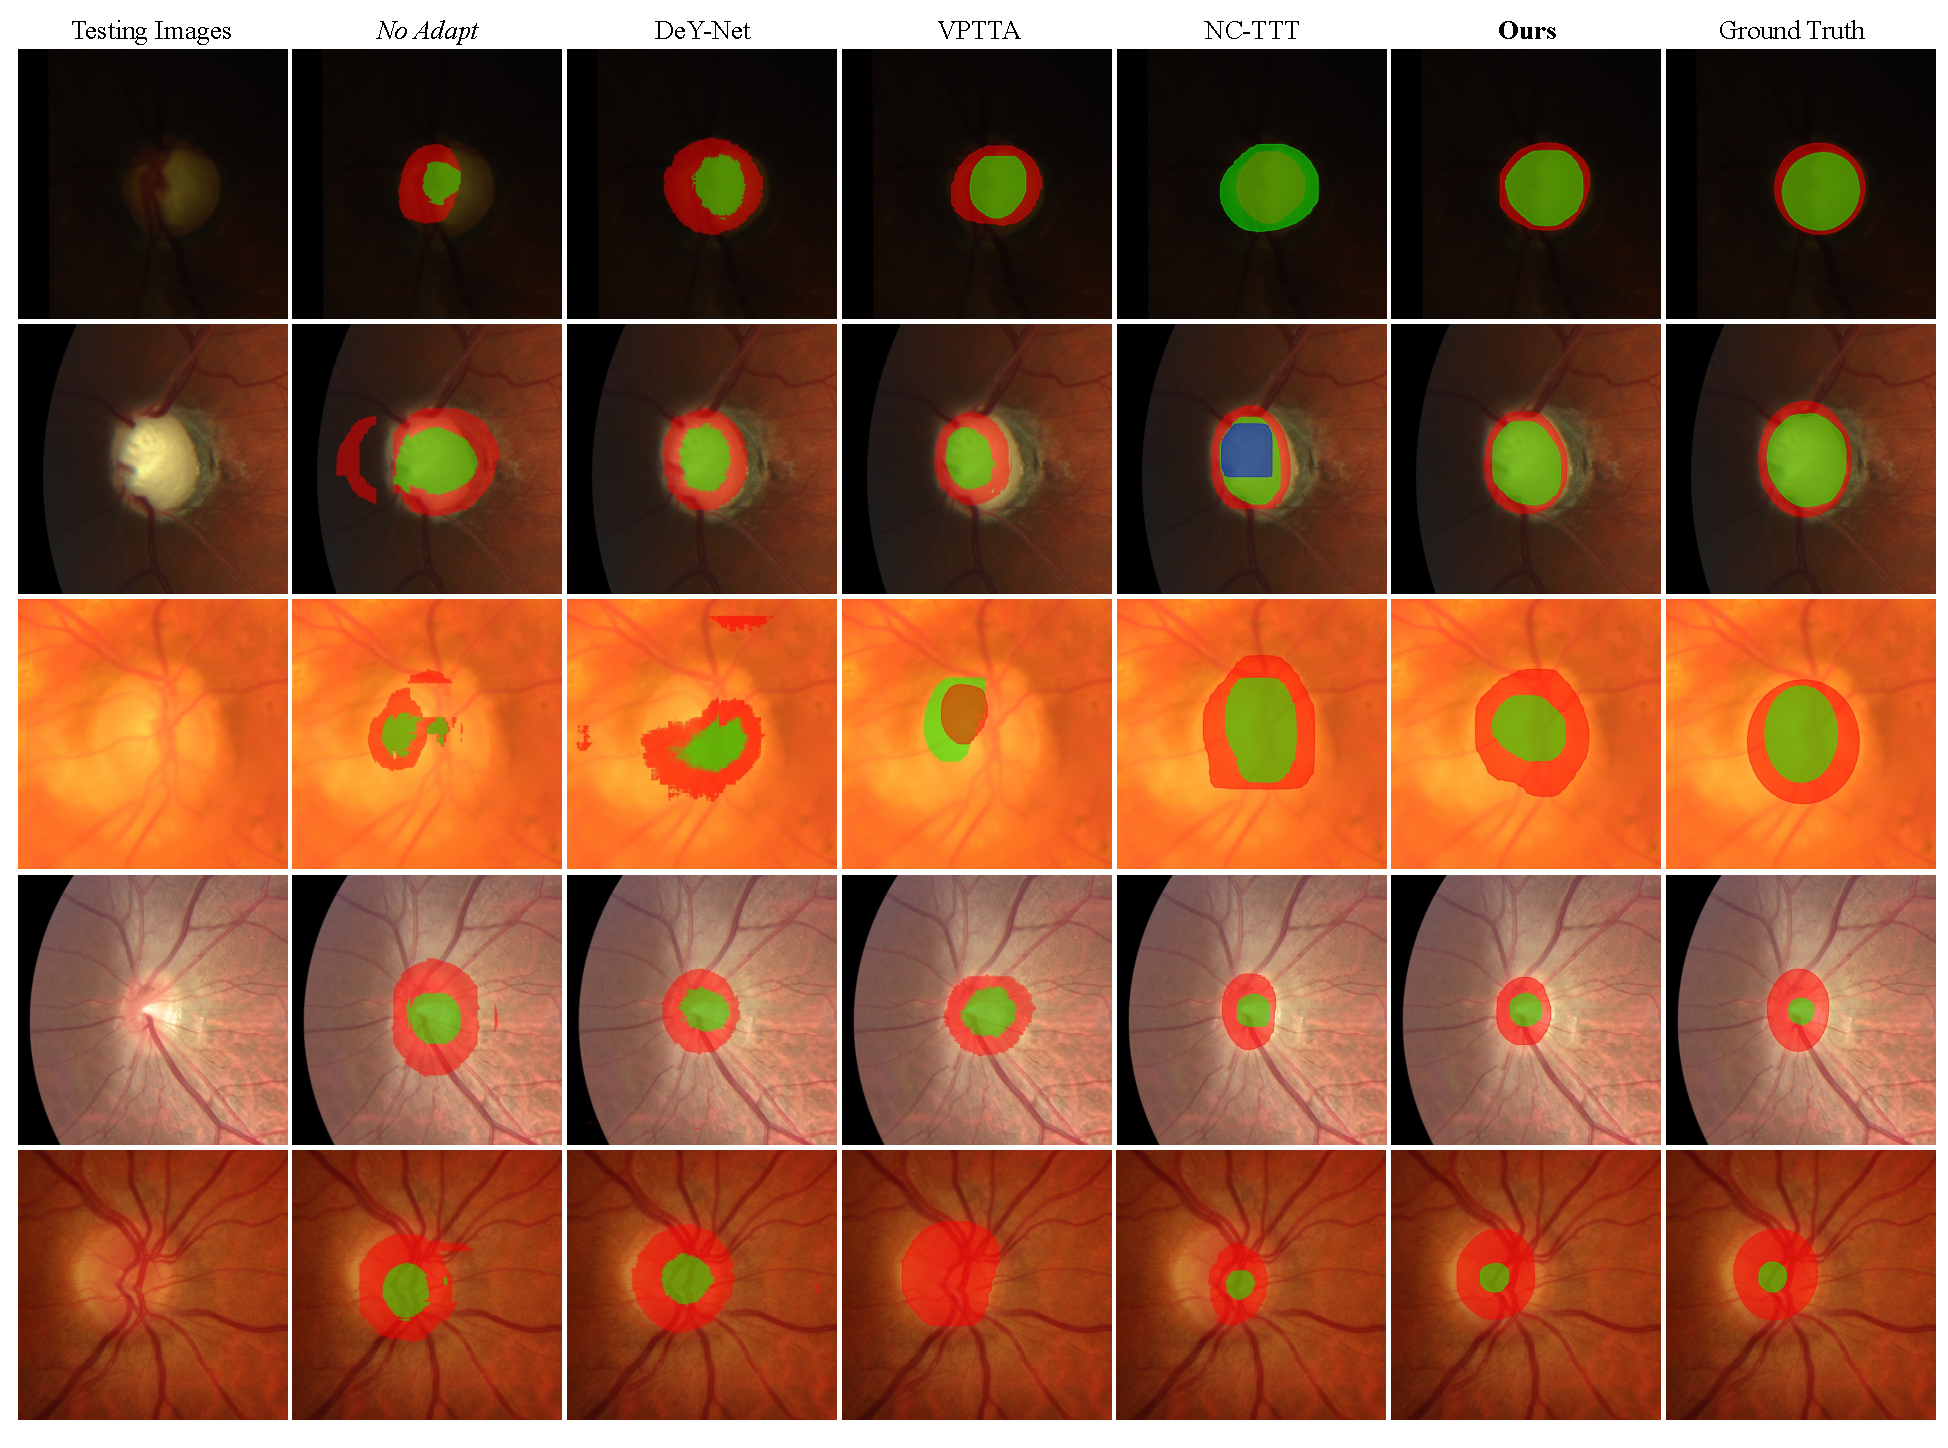
\includegraphics[width=0.999\linewidth]{Figures/visual_com_fundus.pdf}
    % \vspace{-10pt}
    \caption{Visualization comparison of segmentation results for the \textit{No Adapt} baseline, DeY-Net~\cite{wen2024denoising}, VPTTA~\cite{chen2024each}, NC-TTT~\cite{osowiechi2024nc}, and our method in retinal fundus segmentation. The five rows from top to bottom display the final segmentation results for tests conducted on Sites A to E. Different colors represent the segmentation instances of different classes identified by the network.}
     % \vspace{-0.5cm}
    \label{fig:vis_appendix_fundus}
\end{figure*}

\begin{figure*}[!t]
    \centering
    \includegraphics[width=0.999\linewidth]{Figures/visual_com_polyp.pdf}
    % \vspace{-10pt}
    \caption{Visualization comparison of segmentation results for the \textit{No Adapt} baseline, DeY-Net~\cite{wen2024denoising}, VPTTA~\cite{chen2024each}, NC-TTT~\cite{osowiechi2024nc}, and our method in polyp segmentation. The four rows from top to bottom display the final segmentation results for tests conducted on Sites A to D. Different colors represent the segmentation instances of different classes identified by the network.}
     % \vspace{-0.5cm}
    \label{fig:vis_appendix_poloy}
\end{figure*}

Retinal fundus segmentation, in particular, presents a challenge due to the presence of two overlapping substructures. Lower clarity and contrast in images (e.g., rows 1 and 2 of Figure~\ref{fig:vis_appendix_fundus}) further complicate the model’s ability to accurately differentiate and segment these structures. By incorporating morphological priors of the organ within a multi-graph matching network, our method effectively learns robust substructure representations while minimizing domain-related noise. This approach overcomes issues like repeated, missing, or blurred edge pixels commonly seen in other methods, providing a more precise segmentation outcome.

The segmentation of polyps presents a greater challenge than that of retinal fundus imaging due to the highly variable appearance, with marked differences in shape, size, and color across domains. This variability demands precise, pixel-level classification from the network. Furthermore, we have not designated polyp segmentation as a single-object task; the model independently classifies and segments multiple classes during testing, using different colors to distinguish each segmented object in the visualization. As illustrated in Figure~\ref{fig:vis_appendix_poloy}, the masks generated by our method are in close alignment with expert annotations and effectively avoid pixel misclassification into different categories, a common issue in other methods.

\section{Additional Analysis}
\subsection{Effectiveness of the class-wise similarity matrix}
The class-wise similarity matrix $\bold{W}$ is introduced to mitigate category confusion in graphs caused by nodes belonging to different classes. Such confusion often results in mismatches, semantic deviations, and redundant computations. By reordering the adjacency matrix based on the labels $Y_i$ of each node $\mathcal{V}_i$, our method strengthens the capacity to identify and learn class-specific information during the source training phase.
To validate the above perspective, we conducted experiments comparing the final TTA segmentation results with and without $\bold{W}$ (denoted as with $\bold{W}$ and \textit{w/o} $\bold{W}$). As illustrated in Figure~\ref{fig:class_simi_ma}, \textit{w/o} $\bold{W}$ results in a measurable decline in DSC performance. Furthermore, we visualized the effect of \textit{w/o} $\bold{W}$ in multi-object segmentation scenarios, as shown in Figure~\ref{fig:class_w}. While the masks generated by the model closely align with the ground truth, the model misclassified the categories of two segmented instances.

\subsection{Effectiveness of Morphological Priors}
\begin{figure}[h]
    \centering
    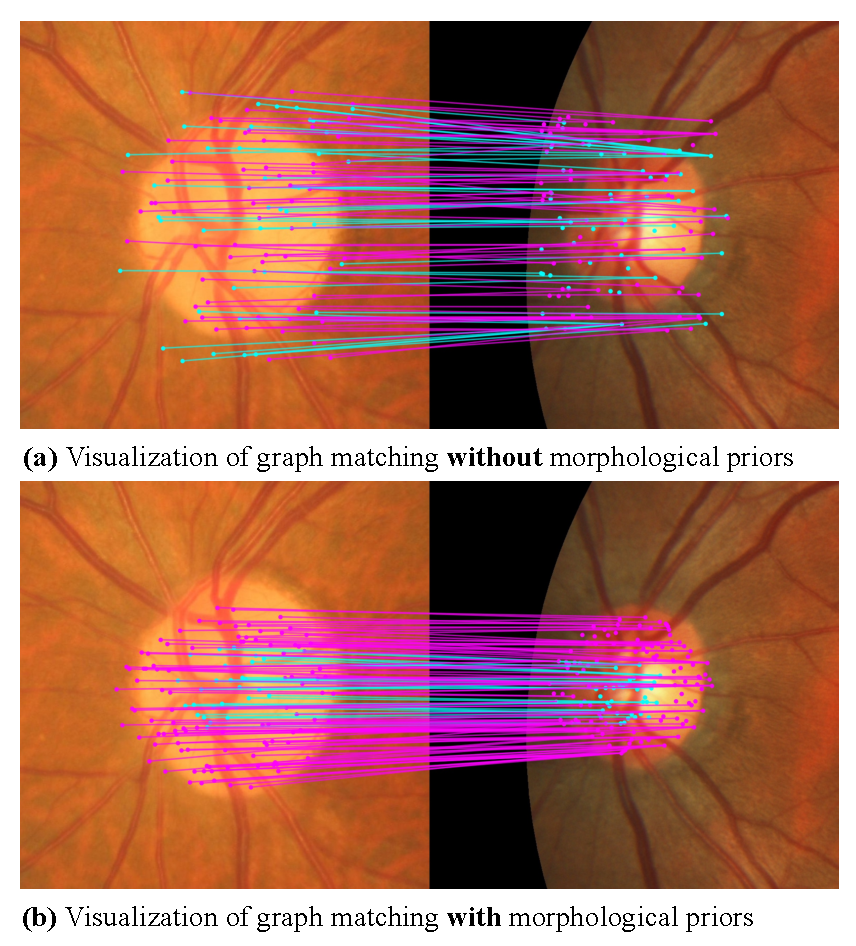
\includegraphics[width=0.999\linewidth]{Figures/visual_pair.pdf}
    % \vspace{-10pt}
    \caption{Visualization of graph pair matching.}
     % \vspace{-0.5cm}
    \label{fig:re_visual}
\end{figure}
We visualized cross-site pairing without morphological priors, as shown in Fig. ~\ref{fig:re_visual}(a), and compared it with the results obtained after incorporating priors, as shown in Fig. ~\ref{fig:re_visual}(b). Without priors, the graph nodes were not correctly sampled within the corresponding organs, leading to mismatches. 
By introducing priors, this issue was effectively resolved, and multigraph matching ensured more stable pairing across multiple domains. For a quantitative evaluation of the impact of without priors, please refer to Table 4 in the main text.

\begin{figure}[!t]
    \centering
    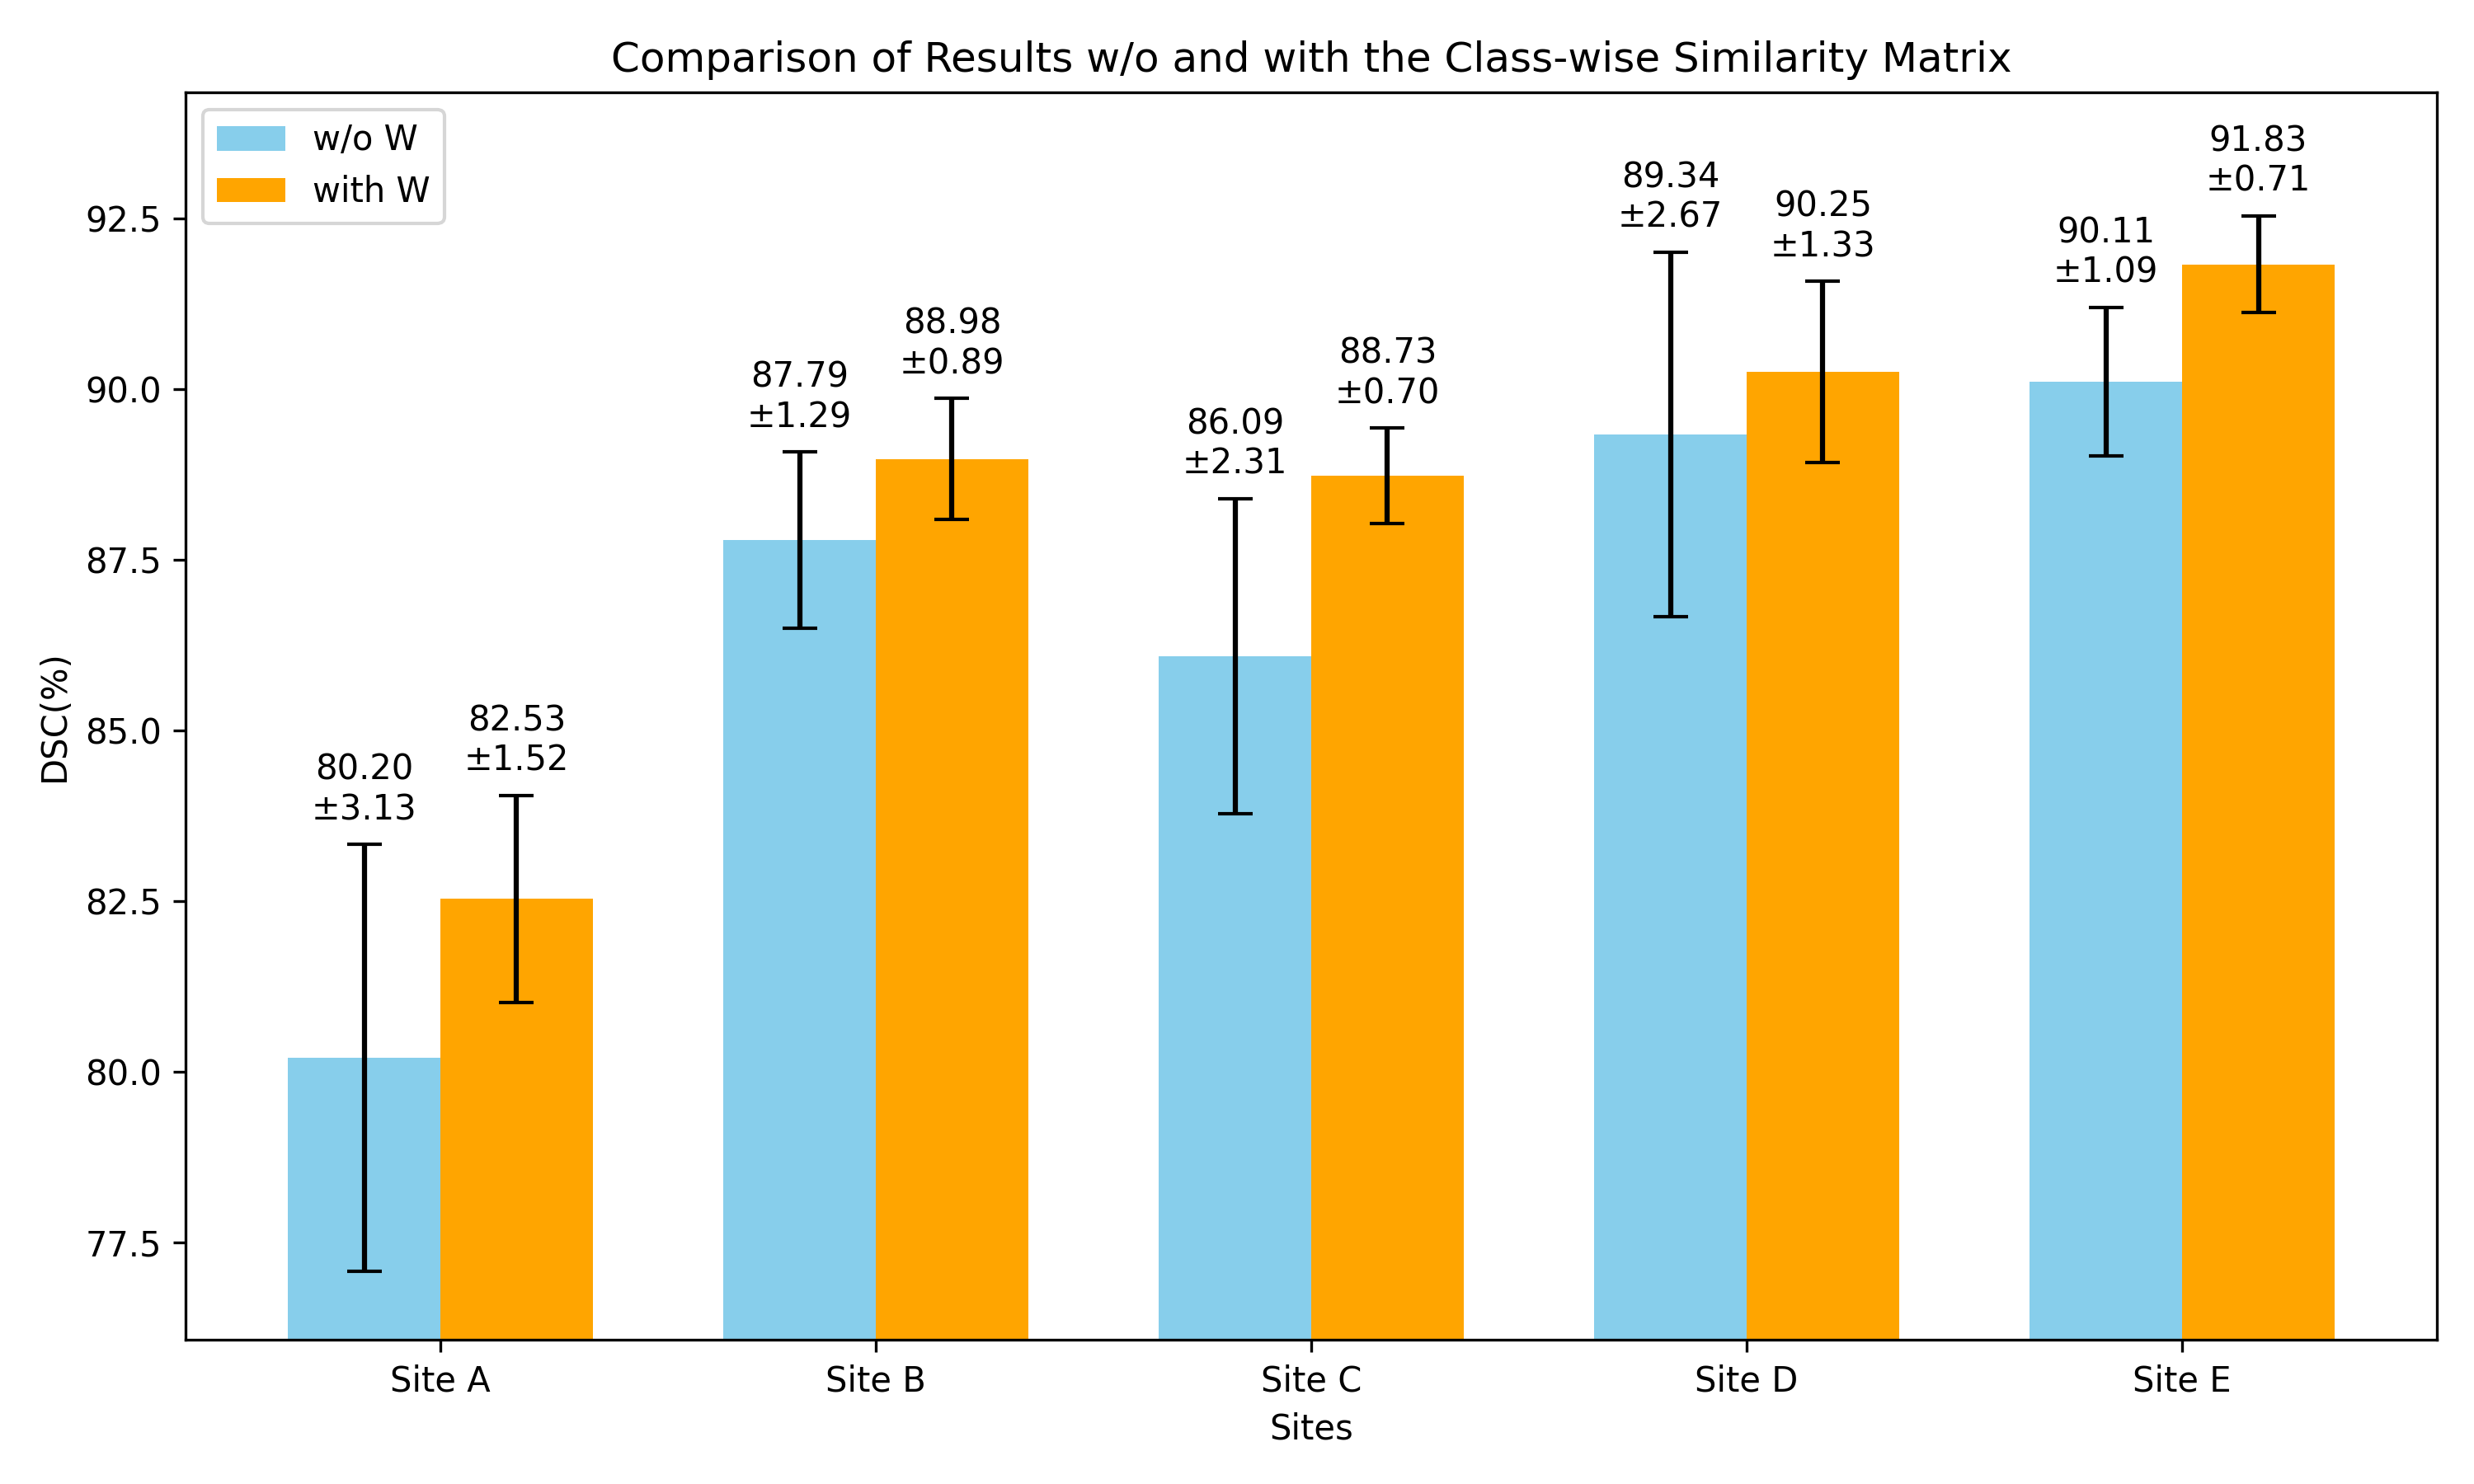
\includegraphics[width=0.899\linewidth]{Figures/class_simi_ma.png}
    % \vspace{-10pt}
    \caption{Ablation study on the impact of the Class-wise Similarity Matrix $\bold{W}$ in retinal fundus segmentation: comparison of results with and without (\textit{w/o}) $\bold{W}$.}
     % \vspace{-0.5cm}
    \label{fig:class_simi_ma}
\end{figure}

\begin{figure}[!t]
    \centering
    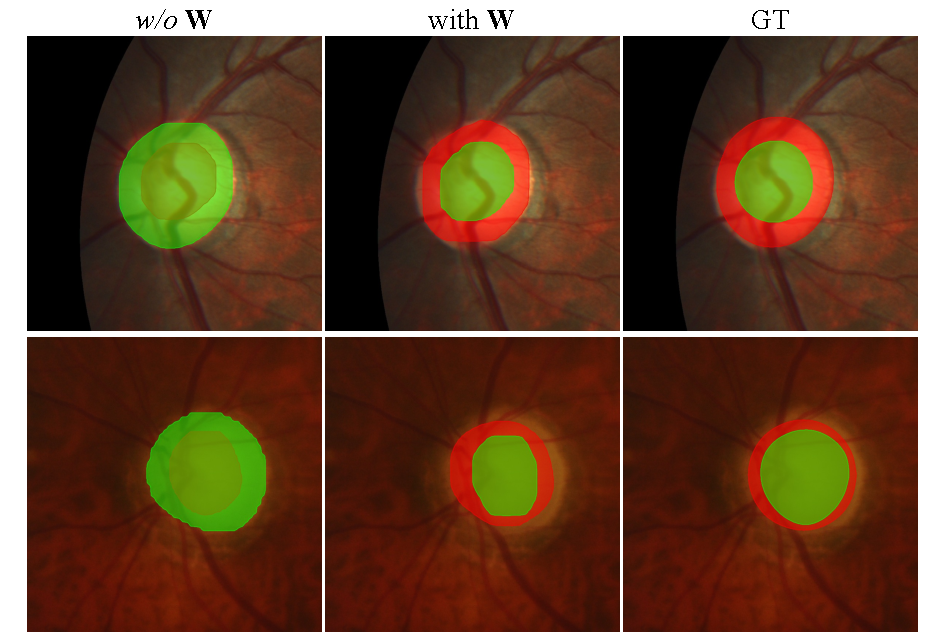
\includegraphics[width=0.999\linewidth]{Figures/visual_class.pdf}
    % \vspace{-10pt}
    \caption{Visualization of segmentation results with and without (\textit{w/o}) the Class-wise Similarity Matrix $\bold{W}$.}
     % \vspace{-0.5cm}
    \label{fig:class_w}
\end{figure}

\subsection{Impact of Batch Size on Segmentation}
\begin{table}[h!]
% \vspace{-9pt}
% \setlength{\tabcolsep}{1pt}
\centering
  \caption{Ablation study on batch size during TTA for retinal fundus segmentation. ``Avg. DSC" represents the average DSC across the five sites, while ``time" indicates the inference time per image.}
  % \vspace{-10pt}
  \begin{adjustbox}{width=0.669\linewidth}
    \begin{tabular}{c|c|c|c}
\hlineB{3}
Batch Size & Avg. DSC & FLOPs (G) & time (s/img) \\ \hline
% \textit{No Adapt} & 69.37 & - & - & - \\
2 & 85.20 & 3.012 & 0.277 \\
4 & 88.46 & 4.255 & 0.392 \\
8 & 88.93 & 20.43 & 0.780 \\
16 & 89.15 & 80.96 & 1.831 \\
32 & 88.31 & 223.1 & 3.715 \\

\hlineB{3}
\end{tabular}
  \end{adjustbox}
  \label{tab:batchsize}
\end{table}

As shown in Table~\ref{tab:batchsize}, increasing the number of simultaneously matched graphs leads to a significant increase in both FLOPs and inference time, while the improvement in segmentation quality remains marginal. To achieve a balance between segmentation performance and computational efficiency, we set the mini-batch size to 4 during the TTA phase in retinal fundus datasets. However, this is a tunable hyperparameter rather than a fixed value, as it depends on factors such as the size of the segmented objects and the input image resolution. Empirically, we find that a mini-batch size between 4 and 8 provides an optimal trade-off.

\section{Limitations}
Unlike mainstream TTA methods that update only the Batch Normalization layers, our approach optimizes all network parameters during test time, achieving superior segmentation performance. However, the increased computational overhead limits deployment on portable devices, making efficiency optimization a key focus for future work.

In our experiments, we also observed that when both large and small organs are present, the model tends to perform better on larger organs while often overlooking smaller ones. This is due to the uniform sampling of foreground nodes, which can lead to diminished segmentation accuracy for small targets. To address this, we plan to incorporate stronger regularization in future work to better guide the sampling and learning of small structures.

Our method is well-suited for medical imaging compared to natural image tasks. In natural images, objects often exhibit significant variation due to intrinsic properties, motion, and state changes. 
% In contrast, organs in medical images remain relatively stable, which aligns well with the prior knowledge.


\begin{algorithm*}
    \caption{\textbf{Source Training Phase per Mini-Batch}}
    \renewcommand{\algorithmicrequire}{\textbf{Input:}}     \renewcommand{\algorithmicensure}{\textbf{Output:}}
    
    \begin{algorithmic}[1]
        \ENSURE 
        $\mathcal{L}_{overall}$: The overall loss for training the segmentation network;

        $\mathcal{U}$: the pre-trained universe embeddings integrate morphological priors;
        

        \REQUIRE 
        $\{ x_i \in \mathbb{R}^{H\times W\times C} \}_{i=1}^m$: A batch of $m$ images from one or multiple domains;

        $\{ y_i \in [0,255] \cap \mathbb{Z} \}_{i=1}^m$: The ground truth masks corresponding to the input images;

        $E(\cdot)$: Feature extractor (ResNet-50);

        $S(\cdot)$: Segmentation head;

        $N$: The total classes number of segmentation organ;

        $\mathcal{U}$: Learnable universe embeddings;
        
        \textit{\textbf{(1) Segmentation Network Training.}}
        \STATE Get the visual feature maps: $f_i \leftarrow E(x_i)$.

        \STATE Get the predict segmentation masks: $\hat{y}_i \leftarrow S(f_i)$.

        \STATE Get the supervised loss: $\mathcal{L}_{sup} \leftarrow \text{CE}(\hat{y}_i, y_i)$, where CE is Cross Entropy Loss.

        \textit{\textbf{(2) Graph Construction.}}
        \FOR{each $i \in [1,m]$}
            \FOR{each object $n \in [1, N]$} 
                \STATE $\{f_{i,k}^n\}_{k=1}^{K} \leftarrow$ Extract feature maps for object $n$ from layers $1$ to $K$ based on $f_i$ and $y_i$.
            \ENDFOR
        
            \STATE Obtain object-specific features: $\{F_{i}^n\}_{n=1}^N \leftarrow Concat(f_{i,1}^n, \dots, f_{i,K}^n)$ for each $n$ in $N$.
        
            \STATE Build features of nodes and corresponding labels: $\{\mathcal{V}_i \in \mathbb{R}^{n_i \times h}, {Y}_i \in \mathbb{Z}^{n_i}\}_{i=1}^m \leftarrow \phi(\{F_i^n\}_{n=1}^N)$, where $\phi$ is the spatially-uniform sampling, and $n_i$ is the total number of nodes for $x_i$. 

            \STATE $ \mathcal{G}_i = (\mathcal{V}_i, \mathcal{A}_i)$, the weighted adjacency matrix $\mathcal{A}_i$ is obtained from Eq. (5).
        \ENDFOR

        \textit{\textbf{(3) Formulation of \textit{universe embeddings}.}}

        \IF{ $\mathcal{U}$ is not initialized}
        \STATE $\mathcal{U} = 1/d + 10^{-3}z$, where $z \sim N(0, 1)$.
        \ENDIF
        \STATE \textit{Universe matching matrices}: $\bold{U} = [U_1^{\mathsf{T}}, \cdots, U_m^{\mathsf{T}}]^{\mathsf{T}}$, where $U_i = Sinkhorn(\mathcal{V}_i \ \mathcal{U}^{\mathsf{T}}, \tau) \in \mathbb{U}_{n_i d}$, $d$ is the \textit{universe size}.

        \STATE Block-diagonal multi-adjacency matrix: $\bold{A} = diag(\mathcal{A}_1, \cdots, \mathcal{A}_m)$. 

        \STATE Compute the class-aware similarity matrix: $\bold{\tilde{A}} = \bold{W}^{\mathsf{T}} \bold{A}\bold{W}$, where $\bold{W} = [W_{ij}]_{ij}$, and $W_{ij} = {Y}_i {Y}_j^{\mathsf{T}}$. 

        \STATE HiPPI solving for stable convergence of $\bold{U}$ as in Eqs. (6-8).

        \STATE Update $\mathcal{U}$ with $L(\mathcal{U})$ in Eq. (9).

        \textit{\textbf{Overall Loss of Source Training.}}
        \STATE $\mathcal{L}_{overall}=\mathcal{L}_{sup}+L(\mathcal{U})$.

% $W_{ij} = {Y}_i {Y}_j^{\mathsf{T}} $ and $\bold{W} = [W_{ij}]_{ij} \in \mathbb{Z}^{(\sum_{i=1}^{m}n_i)\times(\sum_{j=1}^{m}n_j)}$. The class-aware similarity matrix $\bold{\tilde{A}} = \bold{W}^{\mathsf{T}} \bold{A}\bold{W}$.
    \end{algorithmic}
    \label{algo:train}
\end{algorithm*}
% 

\begin{algorithm*}
\caption{\textbf{Higher-order Projected Power Iteration (HiPPI)~\cite{bernard2019hippi}}}
    \renewcommand{\algorithmicrequire}{\textbf{Input:}}     \renewcommand{\algorithmicensure}{\textbf{Output:}}
    
    \begin{algorithmic}[1]
        \ENSURE 
        Cycle-consistent universe-matching $\bold{U}_t$.
        

        \REQUIRE 
        $W$: multi-graph similarity matrix;

        $\bold{U}_0$: initial universe-matching $\bold{U}_0 \in \mathbb{U}_{n_id}$;

        \STATE \textbf{Initialise:} $t\leftarrow 0$, $\text{proj} \leftarrow Sinkhorn$.
        \REPEAT
        \STATE \hspace{1em} $V_t \leftarrow W \bold{U}_t \bold{U}_t^{\mathsf{T}} W \bold{U}_t$.
        \STATE \hspace{1em} $\bold{U}_{t+1} \leftarrow \text{proj}(V_t)$.
        \STATE \hspace{1em} $t\leftarrow t+1$.
        \UNTIL{ $|| U^t_i - U^{t-1}_i|| < 10^{-5}$}
    \end{algorithmic}
\label{algo:hippi}
\end{algorithm*}

\begin{algorithm*}
    \caption{\textbf{Test-time Adaptation Phase per Mini-Batch}}
    \renewcommand{\algorithmicrequire}{\textbf{Input:}}     \renewcommand{\algorithmicensure}{\textbf{Output:}}
    
    \begin{algorithmic}[1]
        \ENSURE 
        $\{y^{*}_i \in \mathbb{R}^{H\times W\times C} \}_{i=1}^m$: The predicted masks of test dataset.
        
        
        \REQUIRE 
        $\{ x_i^t \in \mathbb{R}^{H\times W\times C} \}_{i=1}^m$: A batch of $m$ images from test dataset;

        % $\{ y_i \in [0,255] \cap \mathbb{Z} \}_{i=1}^m$: The ground truth masks corresponding to the input images;

        $E(\cdot)$: Pre-trained feature extractor (ResNet-50);

        $S(\cdot)$: Pre-trained segmentation head;

        $N$: The total classes number of segmentation organ;

        $\mathcal{U}$: Pre-trained learnable universe embeddings;

        \textit{MIter}: Max iteration of multi-graph matching.

        \STATE \textbf{Initialise:} \textit{Iter}$\leftarrow 0$. ${V}_i \leftarrow 0$, $\forall i \in [m]$. ${V}_i$ is the gradient of Eq. (4) with respect to ${U}_i$. $\tau \leftarrow 0.05$.

        \STATE Obtain the visual feature maps: $f_i^t \leftarrow E(x_i^t).$

        \STATE Obtain the pseudo segmentation masks: $\hat{y}^t_i \leftarrow S(f_i^t).$

        \textit{\textbf{(1) Graph Construction.}}

        \STATE $ \mathcal{G}_i^t = (\mathcal{V}_i^t, \mathcal{A}_i^t)$, where $\mathcal{V}_i^t$ and $\mathcal{A}_i$ are obtained in the same manner as in Algorithm~\ref{algo:train}. (2).

        \textit{\textbf{(2) Unsupervised Multi-graph Matching.}}

        \STATE Universe matching of $\mathcal{G}_i$: $U_i = Sinkhorn(\mathcal{V}_i^t \ \mathcal{U}^{\mathsf{T}}, \tau)$.
        % $\bold{U} = [U_1^{\mathsf{T}}, \cdots, U_m^{\mathsf{T}}]^{\mathsf{T}}$, where 

        \FOR{ $(\mathcal{G}_i, \mathcal{G}_j)$ in $\{ \mathcal{G}_1, \cdots, \mathcal{G}_m \}$}
        \STATE Affinity matrix $M_{ij} \leftarrow f_{mlp}\{\mathcal{V}_i^t \mathcal{W}_{x}^t\cdot(\mathcal{V}_j^t \mathcal{W}_{y}^t)^{\mathsf{T}}\}$, where $\mathcal{W}_{x}^t$ and $\mathcal{W}_{y}^t$ are two learnable linear projection, $f_{mlp}$ is a multi-layer perception (MLP).

        \REPEAT

        \STATE $V_i \leftarrow V_i + (\lambda \mathcal{A}_i^t U_i U_j^{\mathsf{T}} \mathcal{A}_j^t U_j + M_{ij} U_j)$.

        \STATE Relax $V_i$ to the space of universe: $U_i \leftarrow sinkhorn(V_i, \tau)$. 

        \UNTIL{$\{U_i\}$ \textit{converged} OR \textit{Iter} $>$ \textit{MIter}}

        \ENDFOR
        
    \STATE Fine-tune the segmentation network (update $E$ and $S$) using $L_{mat}$ in Eq. (12).


    \textit{\textbf{(3) Final Inference Process.}}
    
    \STATE  $y^{*}_i = S(E(x_i))$

    \end{algorithmic}
    \label{algo:test}
\end{algorithm*}

% \clearpage


% {
%     \small
%     \bibliographystyle{ieeenat_fullname}
%     \bibliography{main}
    
% }

